\chapter{Architektur}\label{konzept_1}
\section{Allgemein}
\subsection{Ausgangslage}
Als Rich Client Framework wird Eclipse 3.x\footnote{die aktuelle Version ist 3.7 (stand: 31.8.2011)} genommen. Siehe Abschnitt \titleref{selection_rcp_fw}. In der Folge werden die für die Eclipse Plattform gebräuchlichen Begrifflichkeiten verwendet. 

\subsection{Lizenzierung der Software}
Die Software wird lizenziert unter der Eclipse Public License\footnote{http://www.eclipse.org/legal/epl-v10.html} in der Version 1.0. Dies ist eine freie Software-Lizenz und gewährt das Recht zur freien Nutzung, Weiterverbreitung und Veränderung der Software. Die Benutzung einer Open-Source Lizenz hat insbesondere folgende Vorteile:
\begin{itemize}
	\item An der Entwicklung von Open-Source Software können sich eine beliebige Anzahl an Entwickler beteiligen. Der Entwicklungsaufwand kann skaliert werden.
	\item Jedermann kann Erweiterungen entwickeln oder Fehler beheben.
\end{itemize}

\section{Architektur}\label{konzept_uebersicht}
Aufgrund der Anforderung QRQ-S-01 (Erweiterbarkeit) muss die Analyse-Software auch hinsichtlich anderer Logformate erweiterbar sein. Die Applikation wird also nicht zwingendermassen mit der Erweiterung für JRockit Logdateien verwendet. Es könnte zu einem späteren Zeitpunkt sein, dass man damit Garbage Collection Logs der HotSpot Virtual Machine auswertet. Dies hat hinsichtlich Architektur einige Konsequenzen:
\begin{itemize}
	\item Die Applikation wird in zwei Komponenten aufgeteilt:
		\begin{itemize}
			\item Basissoftware
			\item Erweiterung JRockit
		\end{itemize}
		Die Basissoftware kann unabhängig von den Erweiterungen installiert werden, für die Auswertung einer Logdatei ist allerdings die entsprechende Erweiterung zu installieren. Eine Erweiterung kann ohne Basissoftware nicht gebraucht werden.
	\item Die Architektur der Applikation muss es zulassen, dass zu einem späteren Zeitpunkt auch Garbage Collection Logs von anderen Virtuellen Machinen analysiert werden können.
	\item Die Basissoftware stellt Extension-Points\footnote{Ein Extension-Point ist ein Mechanismus der von Eclipse zur Verfügung gestellt wird, damit eine Komponente (Plugin) sich bei einer anderen registrieren kann.} bereit, über welche sich die Erweiterungen  registrieren.
\end{itemize}

\subsection{Struktur}
Die generischen Aspekte der Software befinden sich in der Basissoftware. Nur die Spezialisierung im Bereich jedes einzelnen Log-Formats findet in den Erweiterungen statt. Grundsätzlich werden die Aufgaben folgendermassen verteilt:
\begin{itemize}
	\item Basissoftware (Core Feature)
		\begin{itemize}
			\item Garbage Collection Log importieren
			\item Garbage Collection Log einlesen
			\item Profil erstellen, speichern, exportieren, importieren
			\item Hilfesystem (wobei allerdings jedes einzelne Feature spezifische Hilfethemen beisteuern kann)
		\end{itemize}
	\item JRockit Extension (JRockit Extension Feature)
		\begin{itemize}
			\item Garbage Collection Log parsen
			\item Jede Erweiterung hat ein eigenes Domänemodell, da der Aufbau des Garbage Collectors Herstellerabhängig ist.
		\end{itemize}
\end{itemize}

Das Core-Feature ist die Basis und verantwortlich für den gesamten Import-Prozess (Import-Wizard, Leseprozess der Log-Datei, Anzeige der Menus, Profil-Verwaltung, etc.). Die JRockit Extension ist eine für die Garbage Collection Logs der JRockit geschriebene Erweiterung. Sie ist für das Parsing der Logdateien, die Aufbereitung und Bereitstellung der Daten zuständig. Beinhaltet aber keine Basisfunktionalität.
 \begin{figure}[H]
  	\centering
    	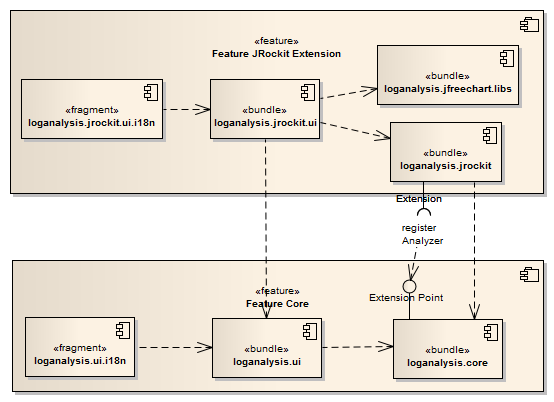
\includegraphics[width=14cm]{images/architektur_komponenten_uebersicht}
        	\caption{Architektur: Komponentendiagramm}
\end{figure}

Das Core Feature besteht aus dem Modul User Interface (``loganalysis.core.ui'') und einem von JFace und SWT\footnote{JFace und SWT wird in Eclipse als Library für die Präsentationsschicht verwendet.} unabhängigen Teil (``loganalysis.core''). Öffnet der Benutzer eine Garbage Collection Logdatei, wird diese durch das Core Feature eingelesen und der Inhalt wird an alle verfügbaren Extensions weitergeleitet. Die erste Extension welche den Inhalt der Datei verarbeiten kann, öffnet seine dafür vorgesehenen Reports und Charts. Jede Extension hat ein basierend auf der Logdatei eigenes Domänen-Modell.

\subsubsection{Nicht-funktionale Module}
Die folgenden Projekte (Plugins) sind im Zusammenhang mit dem Deployment und Testing notwendig, beinhalten aber keine eigentliche Funktionalität. In der Regel beinhalten sie Konfigurationsdateien oder Test-Klassen:
\begin{itemize}
	\item Test-Projekte\footnote{Der Test-Code befindet sich in eigenen Projekten (siehe Abschnit \ref{testing}).}
		\begin{itemize}
			\item core.test
			\item core.ui.test
			\item jrockit.test
			\item jrockit.ui.test
		\end{itemize}
	\item  Features\footnote{Features sind in sich lauffähige Softwarekomponenten mit definiertem Umfang. Zur Defininition wird ein eigenes Eclipse-Projekt erstellt.}
		\begin{itemize}
			\item loganalysis.feature
			\item loganalysis.jrockit.feature
		\end{itemize}
	\item  Thirdparty Bibliotheken\footnote{Thirdparty Bibliotheken werden bei Eclipse-Anwendungen als Plugins gepackt.}
		\begin{itemize}
			\item  loganalysis.jfreechart.libs (JFreeChart Library)
		\end{itemize}
	\item  Targetplattform\footnote{Definiert gegen welche Plattform die Anwendung entwickelt wird.}
		\begin{itemize}
			\item  loganalysis.targetplatform (beinhaltet die Target-Plattform)
		\end{itemize}
	\item  Update-Seite\footnote{Definiert bereitgestellte Features}
		\begin{itemize}
			\item loganalysis.updatesite (definiert und generiert die Update-Seite)
		\end{itemize}
\end{itemize}

\subsection{Verhalten}
\subsubsection{Ablauf Garbage Collection Analyse}
Beim öffnen einer Analyse wird die zuständige Extension gesucht\footnote{Extensions registrieren sich via das plugins.xml an einem Extension-Point. }, welche den Inhalt\footnote{Der Inhalt der Datei wird lazy via die Methode getContent und einem ContentReader geladen.} der Logdatei versteht. Die Erweiterung ist für das Parsen und Aufbereiten der Daten und die Anzeige in einem Analysefenster zuständig. Der Ablauf ist in folgendem Diagramm grafisch illustriert:
 \begin{figure}[H]
  	\centering
    	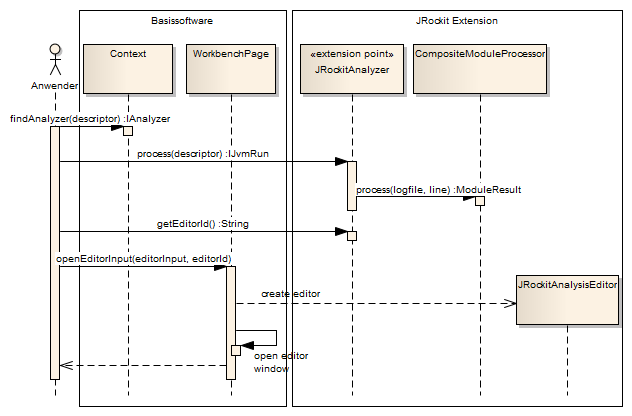
\includegraphics[width=16cm]{images/core_sequence_analysis}
	\caption{Sequenz-Diagramm Öffnen der Analyse}
\end{figure}
Der Ablauf der Garbage Collection Analyse ist folgendermassen:
\begin{enumerate}
	\item Via Context wird die Erweiterung\footnote{Erweiterungen registrieren sich als Extensions an Extension-Points. Diese Konfiguration befindet sich im plugin.xml.} gesucht.
	\item Der Analyser der Erweiterung interpretiert den Inhalt und speichert die Daten im eigenen Domänenmodell.
	\item Der Editor wird geöffnet.
\end{enumerate}

